\documentclass[11]{article}

\usepackage[a4paper,left=3cm,right=2cm,top=2.5cm,bottom=2.5cm]{geometry}
\usepackage{lipsum}
\usepackage{amsmath}
\usepackage{multirow}	
\usepackage{graphicx}


\title{Machine Learning HW2}
\author{Payam AZAD - 503111554}
\begin{document}
\pagenumbering{gobble}
 \maketitle
 
 \begin{table}[ht!]
\centering
\label{my-label}
\begin{tabular}{|ll|l|l|l|l|l|l|}
\hline
                                             &          & Q1 & Q2 & Q3 & Q4 & Q5 & Total \\ \hline
\multicolumn{1}{|l|}{\multirow{2}{*}{Grade}} & Max      & 1  & 1  & 1  & 1  & 1  & 5     \\ \cline{2-8} 
\multicolumn{1}{|l|}{}                       & Expected & 1  & 1  & 1  & 1  & 0  & 4     \\ \hline
\end{tabular}
\end{table}


 \section*{Q1}
 
 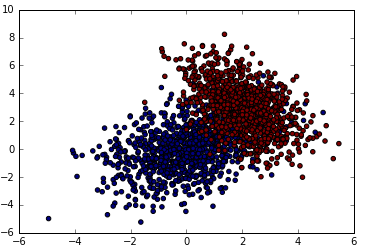
\includegraphics[scale=1]{fig1.png}
 
 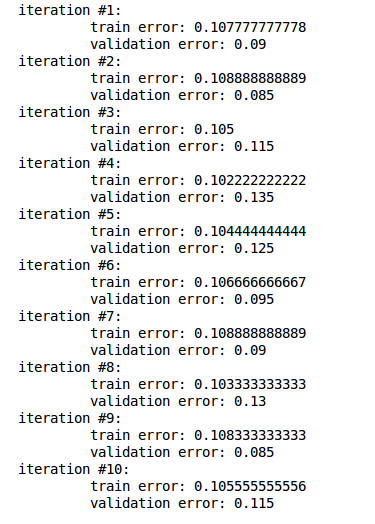
\includegraphics[scale=1]{fig2.png}
 
 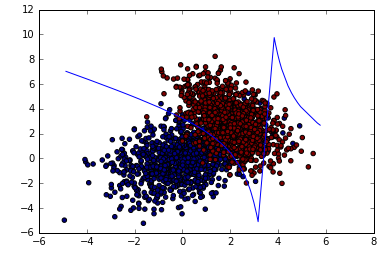
\includegraphics[scale=1]{fig3.png}
\section*{Q2}


 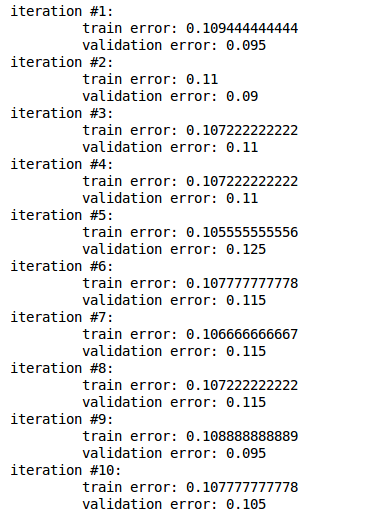
\includegraphics[scale=1]{fig4.png}
 
 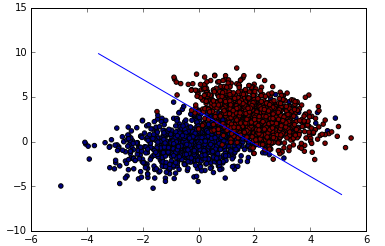
\includegraphics[scale=1]{fig5.png}
 \section*{Q3}

 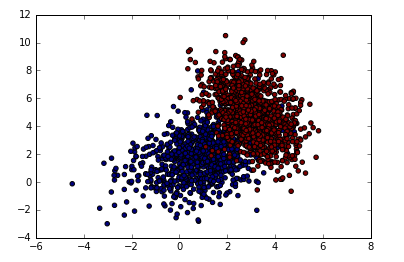
\includegraphics[scale=1]{fig6.png}


 \section*{Q4}


 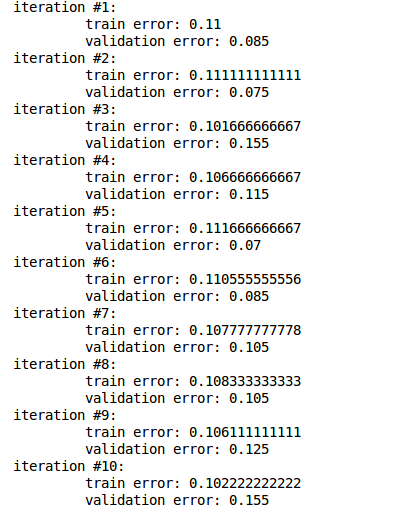
\includegraphics[scale=1]{fig7.png}
 
 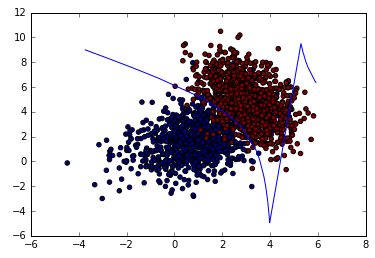
\includegraphics[scale=1]{fig8.png}

 \section*{Q5}




 

\end{document}